\chapter{Experimentation}

This chapter details our experimentation work to answer our key research questions. Each experiment contains an associated objective, approach, results and discussion section. We start our experimentation with our simulation-based experiments, detailing our testing of the LTE standard, and work to understand the link between the handover triggers and the ping-pong rate. We continue our work on the real-world LTE testbed, examining the radio characteristics in various mobility modes and the latency and throughput impacts of a handover event. We compare the changes in response for different cell densities and finally show the relationship between the hysteresis parameter and the handover rate in an indoor setting.

\section{ZMQ-based Handover in srsRAN}
\subsection{Objective}
The first phase aims to understand the basics of handover using srsRAN in a controlled simulation. We can use ZMQ and GNU radio to emulate the radio layer.

\subsection{Approach}
Following \citet{powell_handover_2021}, we started with a pure simulation-based experiment of inducing a handover event. This is accomplished using ZMQ and GNU Radio to simulate the radio layer.

ZMQ\cite{zeromq}, or ZeroMQ, is an asynchronous messaging library that emulates radio transmission. GNU radio\cite{gnuradio} is a software development toolkit that uses ZMQ to interface the various srsRAN components. It also provides signal processing blocks to emulate attenuation between specific radio devices.

\begin{itemize}
    \item We set up the experiment by running an Open5GS network core (EPC), two eNBs, and a UE; the latter two are binaries provided by srsRAN.
    \item The eNBs are connected to the EPC over the S1AP interface over TCP on our local machine.
    \item The eNBs connect to the UE using GNU radio and ZMQ, communicating over various TCP ports.
    \item To emulate propagation loss, we add \texttt{multiply} blocks provided by GNU radio (that amplify or attenuate a signal by some constant) on the send and receive channels from each UE to eNB connection, initially setting it to 1 for the eNB we designate as the source cell and 0 for the ``target" cell. 
    \item We must additionally add a \texttt{throttle} processing block, which keeps the sampling rate consistent with what srsRAN expects.
    \item On the srsUE process, we collect the measurement logs, fetching the RSRP for both cells.
    \item We gradually increase the multiply for the target cell, reducing attenuation until the RSRP is over the hysteresis threshold and the UE is handed over to the target cell.
\end{itemize}

Our GNU radio flowchart is displayed in Figure \ref{fig:gnuradio}. TX is the radio transmission channel, and RX is the receiving channel. The multiply constant blocks are variable and are adjusted during simulation.
\begin{figure}[h]
    \centering
    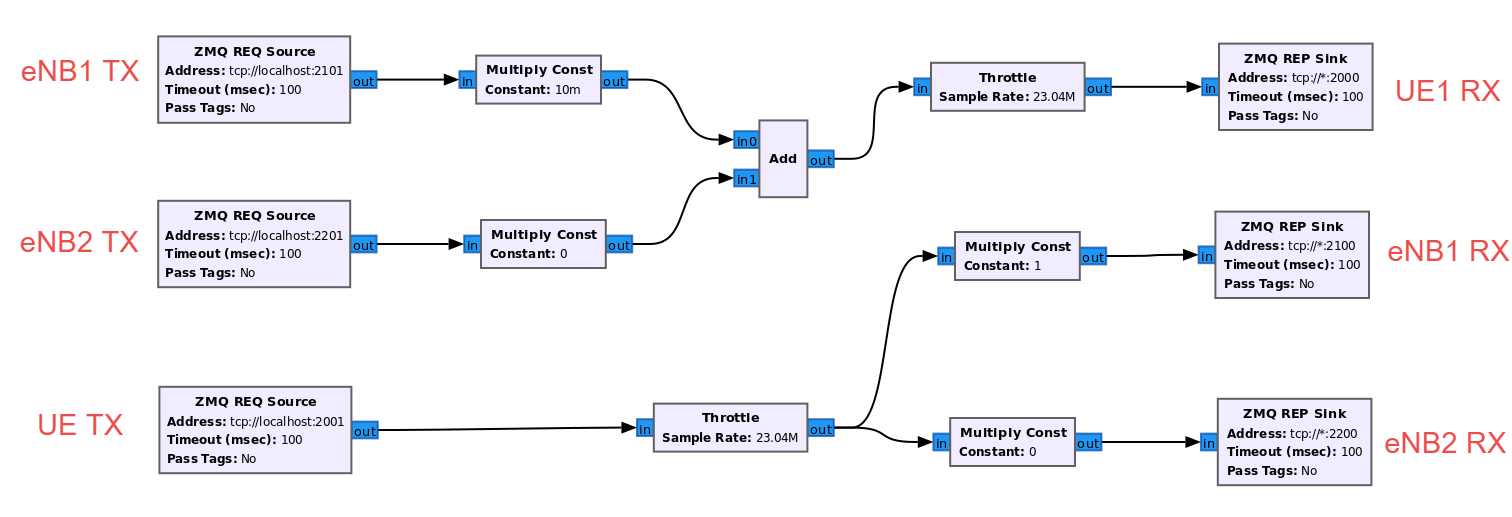
\includegraphics[width=1\linewidth]{src//img/flowchart.png}
    \caption{GNU Radio Handover Flowchart}
    \label{fig:gnuradio}
\end{figure}

\subsection{Results}
Figure \ref{fig:methods:zmq-s1-handover} shows the experiment's results, with the y-axis representing signal strength and the x-axis being a dimensionless attenuation constant. We see handover occurring at -67dBm, 3dBm higher than the connection strength to our source eNB (eNB1). From this, we can see that the hysteresis value in this experiment was 3dBm. 

\begin{figure}
    \centering
    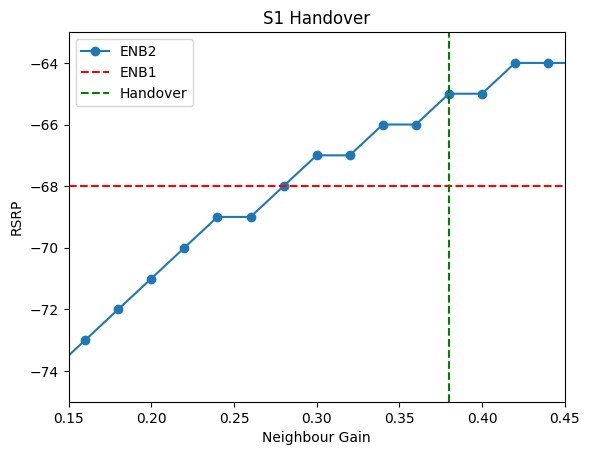
\includegraphics[width=1\linewidth]{src/img/zmq_s1_handover.png}
    \caption{S1 Handover occurring in srsRAN with simulated UE over ZMQ/GNU Radio}
    \label{fig:methods:zmq-s1-handover}
\end{figure}
\subsection{Immediate Discussion}
 srsRAN's default hysteresis parameter (the A3 offset) used in our configuration was 3dBm.  On a static source analysis of the srsRAN source code, we see the handover occurs when the following condition is met:
 \begin{equation}\label{eq:hysteresis}
     \text{RSRP}_\text{Target} - \text{RSRP}_\text{Source} > \text{Hysteresis} + \text{A3 Offset} + \text{Of} + \text{Oc}
 \end{equation}
% $$\text{RSRP}_\text{Target} - \text{RSRP}_\text{Source} > \text{Hysteresis} + \text{A3 Offset} + \text{Of} + \text{Oc}$$
where 
\begin{equation}
\begin{split}
\text{Of} &= \text{Frequency Offset\textsubscript{Target}} - \text{Frequency Offset\textsubscript{Source}} \\
\text{Oc} &= \text{Cell Offset\textsubscript{Target}} - \text{Cell Offset\textsubscript{Source}}
\end{split}
\end{equation}

where in the default setup, $\text{Of}=0$ and $\text{Oc}=0$.

The hysteresis in this equation should not be confused with the hysteresis mentioned in this paper. Instead, it is an additional threshold parameter provided by srsRAN. Together with the A3 offset, this parameter forms the hysteresis trigger parameter discussed in this paper. By default, this parameter is 0dBm, giving us a combined hysteresis value of 3dBm.

This phase confirmed srsRAN's adherence to the LTE standard, and a handover was successfully performed in a simulated environment. This phase was limited by the simplistic nature of the simulated radio network, as constants purely dictated network strength. The limited nature of the simulated environment prompted questions about how handovers would occur in more complex environments.

\section{Custom Network Simulator for Large Scale Handovers}
\label{sec:exp:custom}
\subsection{Objective}
Building on the initial findings, this phase was focused on understanding the ping-pong metric and the associated triggers, employing a custom large-scale simulator for analysis.

\subsection{Approach}
Inspired by \citet{hatipoglu_handover-based_2020}, we reconstructed their non-disclosed tool to simulate large-scale handovers. This allows us to understand better how large-scale handovers are conducted. We can then attempt to replicate their findings to understand what causes ping-pong.

To model handover, we can simplify the modelling to the 2D domain, as vertical propagation loss can be discounted compared to the horizontal propagation between a UE and an eNB. This propagation loss is modelled using the log-distance path loss model\citep{sun_path_2015}:

\begin{equation}
     L=L_{\text{Tx}}-L_{\text{Rx}}=L_{0}+10\gamma \log _{10}{\frac {d}{d_{0}}}+X_{\text{g}}
\end{equation}
Where $L$ is the path loss in decibels, $L_{TX}$ is the transmission power level, $L_{RX}$ is the received power level, $L_0$ is the path loss at the reference distance $d_0$, $d$ is the length of the path, $d_0$ is the reference distance, $\gamma$ is the path loss exponent and $X_g$ is a normal random variable representing the attenuation due to shadow fading (where obstacles affect wave propagation). The values of $L_0$, $\gamma$, $d_0$ and $X_g$ depend entirely on the specific deployment environment, carrier frequency and height of the antenna. We must choose a set of reference values to conduct our experiment.

We reconstruct the same environment as \citet{hatipoglu_handover-based_2020} in Figure \ref{fig:methods:grouped-uesim} to simulate a radio network. The three hexagons represent the movable area, the black squares represent macro-eNBs (lower frequency and higher range), and the black triangles represent the micro-eNBs (higher frequency but lower range). Each coloured dot represents a UE, with the colour representing which eNB it is connected to. The axes units are in meters.

We can simulate UE movement by categorising each UE as a pedestrian, a stationary person, or a vehicle, each of which moves at different speeds. The movement is simulated in timesteps, where at each timestep, a UE can change its heading by a random angle from -10 to 10 degrees.

Handover is calculated using the standard hysteresis and TTT parameters. We simulate different parameters and calculate the percentage of handovers classified as ping-pong, which we define for this experiment as if a handover occurs back to the source cell within 1 second.

\begin{figure}
    \centering
    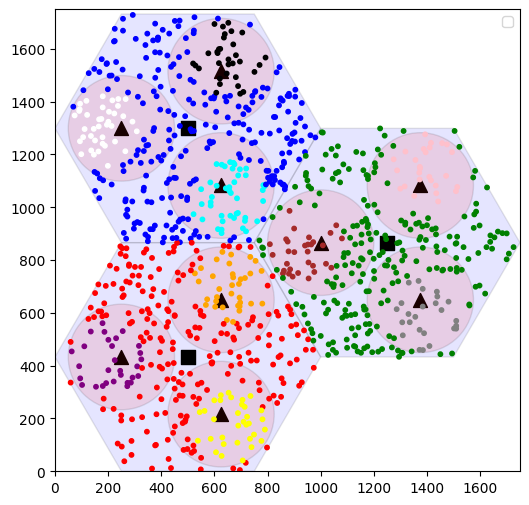
\includegraphics[width=0.75\linewidth]{src//img/grouped_uesim.png}
    \caption{An overview of the 2D simulator}
    \label{fig:methods:grouped-uesim}
\end{figure}
\subsection{Results}
We run the experiment with various handover parameters in Figure \ref{fig:methods:pingpong-uesim}. This graph shows an apparent exponential increase in ping-pong probabilities for a decreasing hysteresis (handover margin). At the same time, the TTT parameter does not provide a noticeable change to the ping-pong probabilities. At a 0dBm hysteresis value, the ping-pong probability reaches 90\%.
\begin{figure}
    \centering
    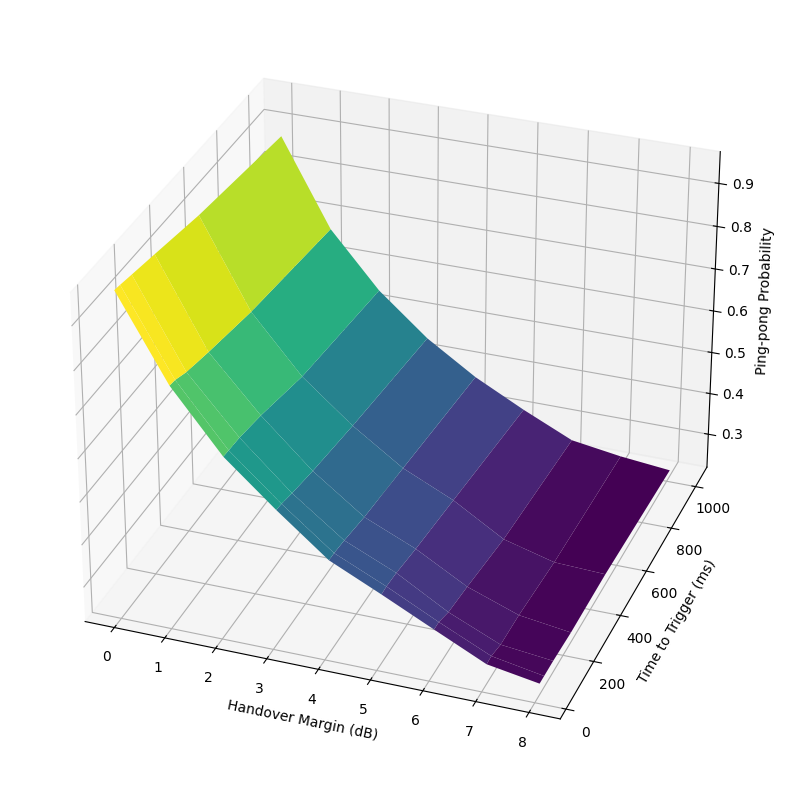
\includegraphics[width=0.5\linewidth]{src//img/custom_pingpong.png}
    \caption{Ping Pong vs Hysteresis and TTT}
    \label{fig:methods:pingpong-uesim}
\end{figure}
\subsection{Immediate Discussion}
The simulator offered some insights into the conditions that cause ping-pong handovers; however, this was majorly limited by the rudimentary nature of the loss propagation function and highly approximate human movement. This reiterates the need for real-world testing to validate these findings, leading to our next experimentation phase.


\section{Real-world Network Testbed Implementation}

\subsection{Objective}
After performing the initial experiments in a simulator, we move on to testing in the real world to validate our simulation insights and provide real insight into indoor scenarios. We use a network of radio-enabled NUCs running as srsENBs to examine handover behaviour in a physical environment.

\subsection{Approach}
We plan on performing a range of experiments using the setup described in Sections \ref{sec:research-lab-layout} and \ref{sec:research-software-stack}. These experiments are outlined in the following subsections.

\subsection{Mobility Tests}
\label{sec:exp:real:mobile}
\subsubsection{Objective}
We wish to examine the performance of the indoor handover in various mobility settings.
\subsubsection{Approach}
To reduce confounding variables, we start the network with only two eNBs for this experiment. We examine four different mobility settings:
\begin{description}[style=unboxed]
    \item[\textbf{Stationary}] We set up this experiment by placing the UE machine between the two eNBs and taking care of the environment remaining entirely static; the UE remained stationary, and no persons moved during the experiment. Here, we expect no handover and that the radio signal (as measured by RSRP) remains constant.
    \item[\textbf{Walking}] We set up this experiment by initially starting the data recording when the UE is near one eNB and then walking towards the other side of the room with the second eNB. Once we reach the eNB, we return to our initial position. To eliminate external factors, no other person was in the lab, and the movement speed was kept roughly constant. We expect the signal strength of the UE to vary proportionally to the distance we are from them and expect a handover to occur once we have moved beyond halfway between the UEs. We expect a second handover on the way back.
    \item[\textbf{Rotating}] This experiment was devised to determine the impact of the angle of UE on the corresponding signal strength. We enable two eNBs on the same wall and place the UE halfway between the eNBs in the centre of the room. We slowly rotate the USRP between the two eNBs, back and forth. We expect no significant change in the signal quality, as LOS is not lost, and the distance between the UE and eNBs does not change.
    \item[\textbf{Dynamic Environment}] In this experiment, we aim to test the network's response to a more dynamic environment. The UE is placed in the same position as the \textbf{Rotating} experiment, facing towards the eNBs' midpoint. During the experiment, a person walks in front of the UE and back again, simulating people walking around in a room. We expect some small drop in the signal strength as LOS with the corresponding eNBs is lost, but we believe that signal reflections contribute a sufficient proportion of the signal strength.
\end{description}
\subsubsection{Results}
The real-world experiments and the description of the experiment are set out in Figure \ref{fig:methods:real-world-testbed}. Here, the plots have an x-axis representing time and a y-axis with the signal strength (RSRP) measured in dBm. Each line plot represents the signal quality between the UE and a specific eNB; in this case, we have two line plots as we have two eNBs. The background colour of the plot represents the eNB to which the UE is currently connected. We have matched the colour palettes (darker shade for the signal quality and pastel shade for the connection) to make the plot more intuitive.
\begin{figure}[p]
    \centering
    \caption{Real-world Network Testbed Implementation: A series of experiments illustrating various aspects of handover behaviour in a real-world setup.}
    \label{fig:methods:real-world-testbed}
    \begin{minipage}{0.45\textwidth}
    \begin{subfigure}{\linewidth}
        \centering
        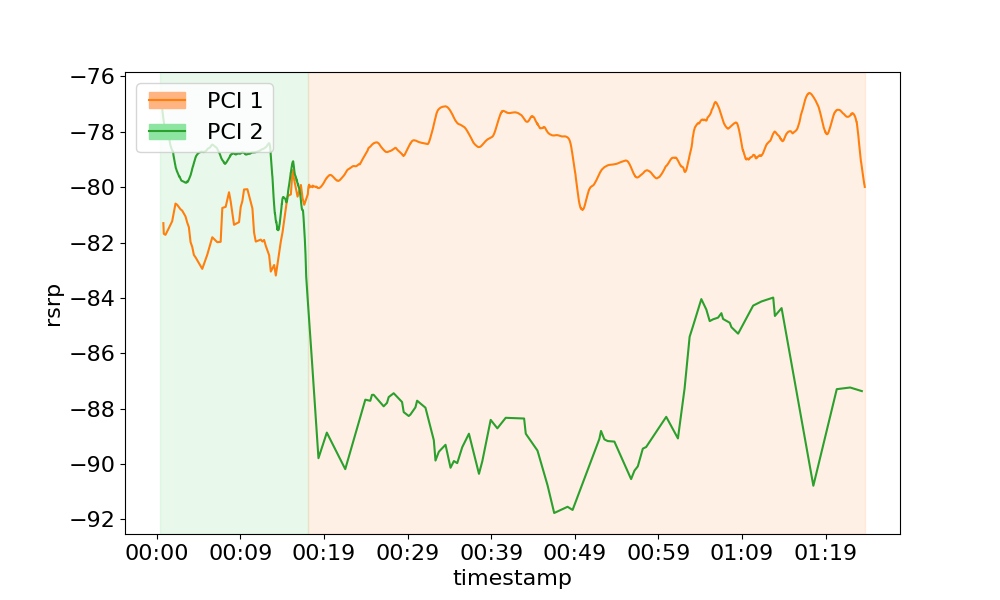
\includegraphics[width=0.9\linewidth]{src/img/real_mobile_2.png}
        \caption{Stationary}
        \label{fig:real:mobile:wait}
    \end{subfigure}
    \end{minipage}
    \begin{minipage}{0.45\textwidth}
        \small{Figure \ref{fig:real:mobile:wait}: Shows the effect of no movement on RSRP measurements, indicating the presence of environmental noise and its potential impact on handover decisions.}
    \end{minipage}
    
    \vspace{1cm}
    \begin{minipage}{0.45\textwidth}
    \begin{subfigure}{.9\linewidth}
        \centering
        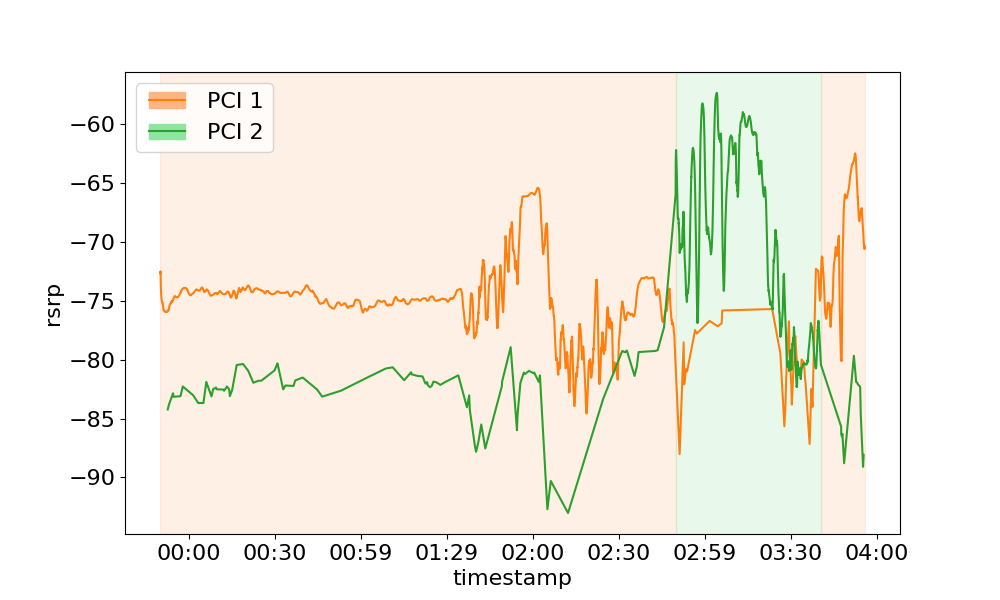
\includegraphics[width=0.9\linewidth]{src//img/real_mobile_0.png}
        \caption{Walking back and forth}
        \label{fig:real:mobile:walk}
    \end{subfigure}
    \end{minipage}%
    \begin{minipage}{0.45\textwidth}
        \small{Figure \ref{fig:real:mobile:walk}: Demonstrates the RSRP and connected cell for a walking back and forth episode. This experiment showcases the dynamic RSRP changes as the UE moves closer or further from each eNB.}
    \end{minipage}
    
    \vspace{1cm}
    \begin{minipage}{0.45\textwidth}
    \begin{subfigure}{\linewidth}
        \centering
        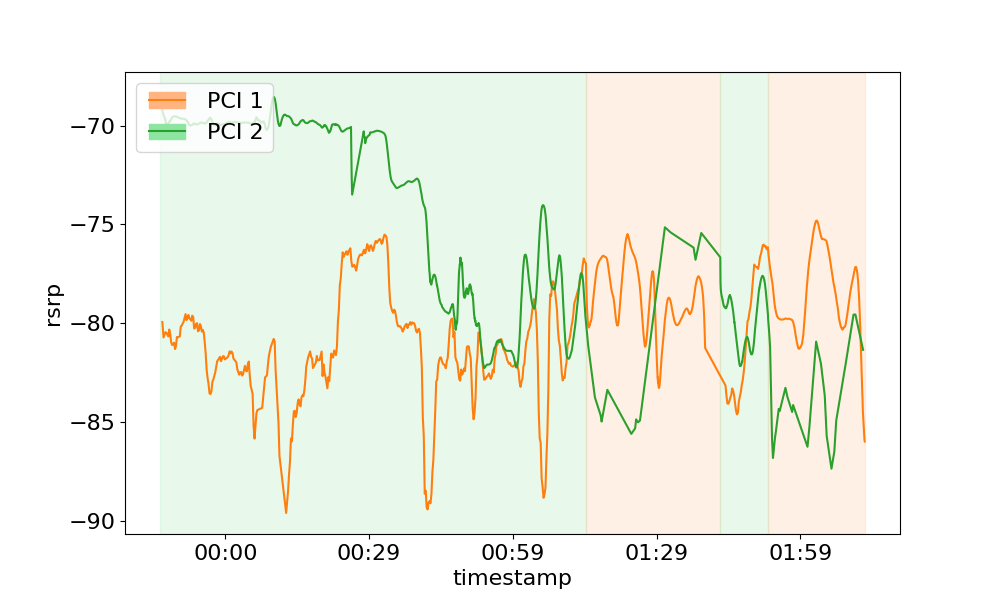
\includegraphics[width=0.9\linewidth]{src//img/real_mobile_1.png}
        \caption{Rotating UE}
        \label{fig:real:mobile:rotate}
    \end{subfigure}
    \end{minipage}
    \begin{minipage}{0.45\textwidth}
        \small{Figure \ref{fig:real:mobile:rotate}: Illustrates the impact of rotating the UE on RSRP fluctuations and handover events, highlighting the sensitivity of handover mechanisms to device orientation.}
    \end{minipage}
    
    \vspace{1cm}
    \begin{minipage}{0.45\textwidth}
    \begin{subfigure}{\linewidth}
        \centering
        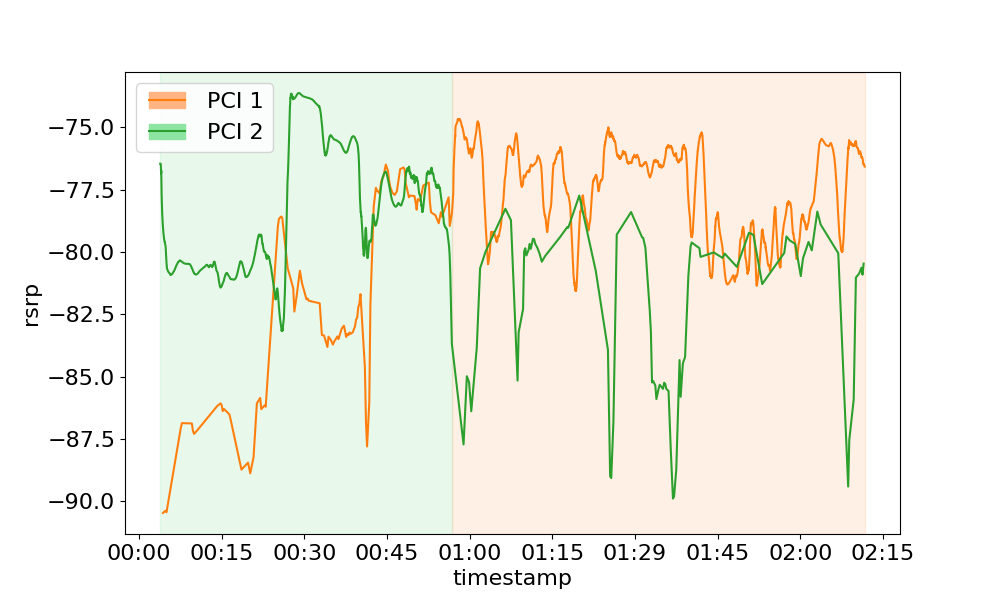
\includegraphics[width=0.9\linewidth]{src//img/real_mobile_3.png}
        \caption{LOS Blockage by walking around}
        \label{fig:real:mobile:block}
    \end{subfigure}
    \end{minipage}
    \begin{minipage}{0.45\textwidth}
        \small{Figure \ref{fig:real:mobile:block}: Examines the effects of line-of-sight (LOS) blockage by simulating movement around the UE. This scenario reflects real-world dynamics where human movement can influence signal quality and handover behaviour.}
    \end{minipage}
\end{figure}
\subsubsection{Immediate Discussion}
These findings underscored the complexity of indoor scenarios.

Figure \ref{fig:real:mobile:wait} shows the high impact of environmental noise even in stationary situations. We expected the RSRP values to remain constant, as the distances between the eNBs and the UE were unchanged, but this was not the case. We observe that even in stationary environments, RSRP can have significant changes, which can trigger handover, as seen at 00:17. The large drop in RSRP at 00:17 for PCI 2 causes PCI 1 to have a greater signal strength over the hysteresis value, causing the eNB to trigger a handover command. We can hypothesise that there are additional second-order effects on signal quality indoors, including environmental noise. 

Figure \ref{fig:real:mobile:walk} shows the network's response as a UE moves linearly between two eNBs. We expect the RSRP to scale smoothly as the UE reduces the distance to a new eNB and reduces as a UE moves away proportionally. We see the expected change in RSRP, including the expected handovers when we moved between the eNBs. There is a handover once the UE approaches the second eNB and another once it returns to the initial eNB. However, the large noise spikes were not accounted for in the expectations of the experiment, where the RSRP does not necessarily scale proportionally. Instead, we see a very noisy, erratic response. 

This is partially explained by Figure \ref{fig:real:mobile:rotate}, where we seek to highlight this possible disparity by rotating the UE back and forth to determine if the angle of the UE would additionally impact the results, causing significant disturbances to RSRP. We indeed see this, as in the figure, the RSRP values fluctuate as we rotate the UE back and forth. This does not change the distance between the network devices. Additionally, this impact on RSRP is significant enough that we see multiple handovers occurring at 01:11, 01:42 and 01:51. 

For the final figure, Figure \ref{fig:real:mobile:block}, we investigate whether LOS blockage could also be an extenuating factor in our previous results. Indeed, we see very large RSRP drops as we move between the UE and the eNB.

The four experiments together highlight the high difficulty of indoor handover. The RSRP values change very quickly and do not behave as expected. We see the relationship between RSRP and distance. However, we see greater than-expected influences from the angle of the UE and the impact of LOS blockage. These combine to form a challenging environment for indoor handover to be controlled and calibrated.

\subsection{Handover Impact on Latency}
\label{sec:handover-impact}
\subsubsection{Objective}
To understand the severity of the issues found in the previous experiment must be mitigated, we must understand the impact on metrics such as throughput and latency of the connection during a handover event. This experiment focuses on the latency introduced by an individual handover.

\subsubsection{Approach}
To determine the latency impact of a handover event, we utilise ICMP \texttt{ping} messages. We set up the UE to send ping messages to the EPC every 10ms. We simultaneously use \texttt{tcpdump}\cite{tcpdump} to capture all incoming and outgoing packets. We then can use Wireshark\cite{wireshark} to analyse the return trip time (RTT). We use Wireshark's inbuild graphing tool to produce a time series of the maximum RTT.

% \begin{itemize}
%     \item To determine the actual impact of a handover, we must measure it quantitatively
%     \item We run a ping flood from the UE to the EPC and capture the packets using `tcpdump`
%     \item Similarly to the previous experiment, we walk from one eNB to another to induce handover
%     \item The packet traces are then analysed with Wireshark to see the latency of each packet. We perform a rolling max smoothing with a window size of 2ms.
%     \end{itemize}

To capture a handover event, we set up the experiment similarly to Section \ref{sec:exp:real:mobile}'s walking experiment, walking from one eNB to the other.
\subsubsection{Results}
The results are shown in Figure \ref{fig:methods:ping-handover}.  We see a significant latency spike during both handover events; however, no packets were dropped due to the EPC/eNB buffering of any packets received during HO. We can see that the latency spike reaches 95ms. 
\begin{figure}
    \centering
    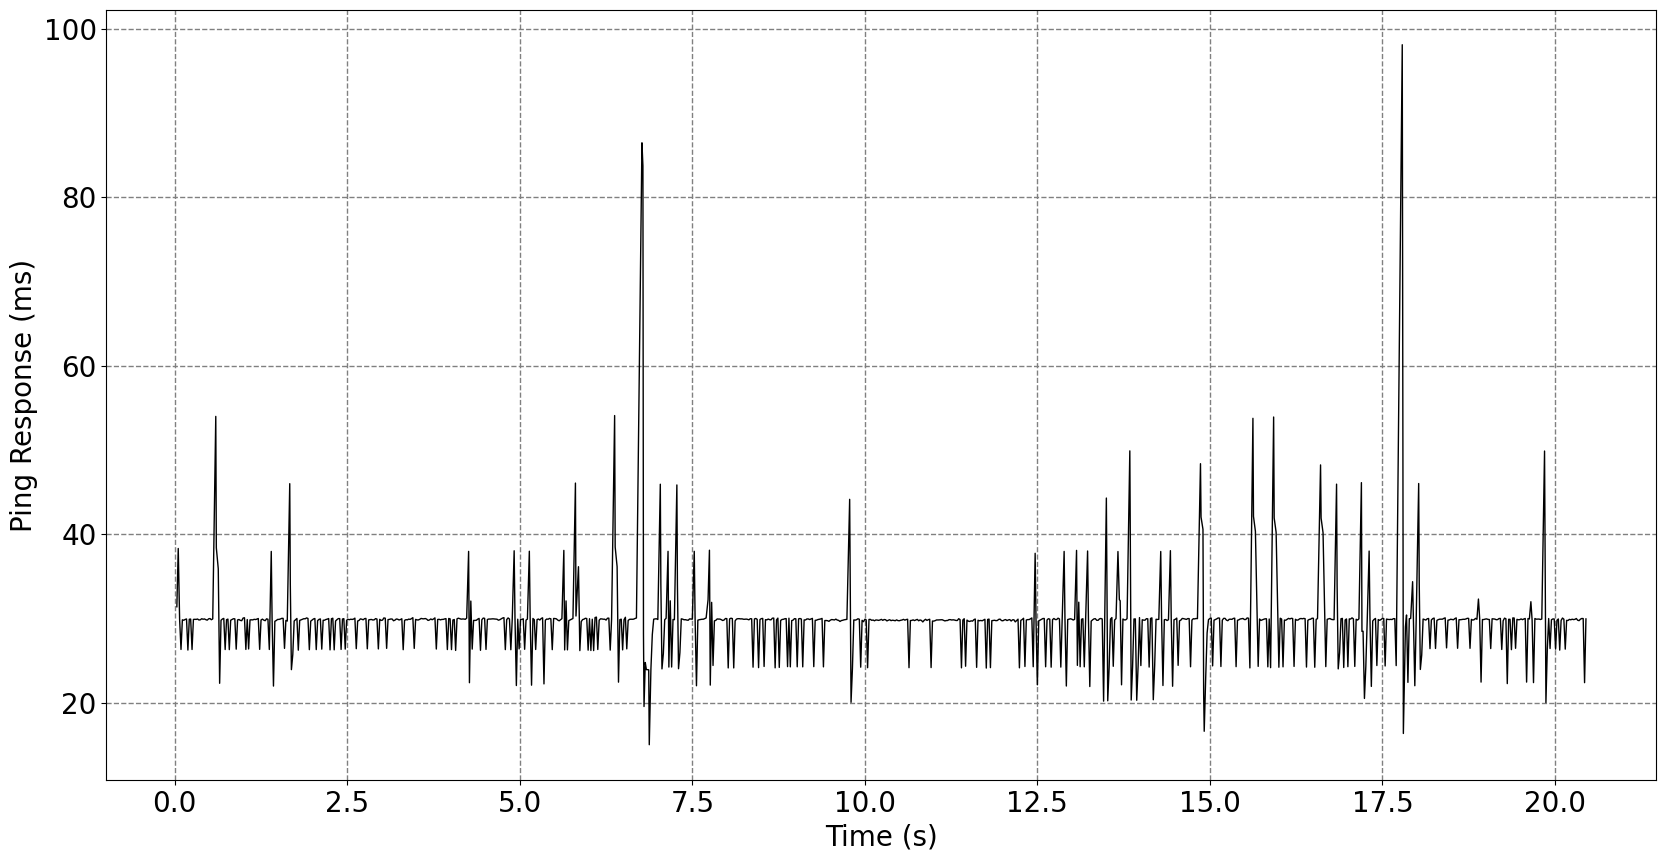
\includegraphics[width=0.75\linewidth]{src//img/ping-handover-hd.png}
    \caption{Ping latency during a handover event}
    \label{fig:methods:ping-handover}
\end{figure}

\subsubsection{Immediate Discussion}
This result is consistent with \citet{zhang_performance_2012}. We understand that the UE will experience a latency penalty for each handover event. This spike in latency does not last long, though, minimising the total impact on the network performance.

\subsection{Throughput Analysis in Indoor Environments}

\subsubsection{Objective}
To further understand the impact of handover in indoor environments, we must also examine the throughput drop due to handover. This section focuses on repeating the mobility tests in Section \ref{sec:exp:real:mobile} while measuring throughput.

\subsubsection{Approach}
We must first determine an approach to measuring the impact on throughput during a handover event. We have two communication protocol options: UDP and TCP. UDP is a best-effort protocol that does not contain rate limiting or reliable message delivery; however, it can deliver the highest throughput. Conversely, TCP ensures reliable message delivery and varies the transmission bandwidth depending on packet loss. It also accounts for the majority of internet traffic. 

We can use the \texttt{iperf3} tool, which is the most popular network performance tester software. It also allows both UDP and TCP testing.

\begin{itemize}
    \item We can set up the experiment by enabling all our eNBs and using our lab machine as a UE. We keep the environment and UE static during the experiment.
    \item We start an \texttt{iperf3} server on the EPC. Simultaneously, we begin a \texttt{tcpdump} process to capture all incoming packets
    \item For testing UDP throughput, we start a client on the UE in UDP mode. We set the bandwidth to 100Mbits/s to saturate the uplink.
    \item For TCP testing, we start the client in TCP mode. The TCP protocol automatically determines the bandwidth.
    \item We can then measure the throughput by examining the lengths of the incoming packets to the EPC.
\end{itemize}

\subsubsection{Results}
Figure \ref{fig:4udp} shows a 30-second capture of UDP throughput. The RSRP values remain constant, while the throughput is very erratic. 

Figure \ref{fig:4tcp} shows 30 seconds of TCP throughput capture. The RSRP values are slightly different. However, the connected eNB has a higher signal strength than the UDP. The throughput is much more constant - due to the TCP rate limiting the connection. However, it transmits at a much lower rate than the UDP connection. Furthermore, connection outages lasting more than 2.5 seconds are caused by the TCP backoff after a radio failure.

\begin{figure}
    \centering
    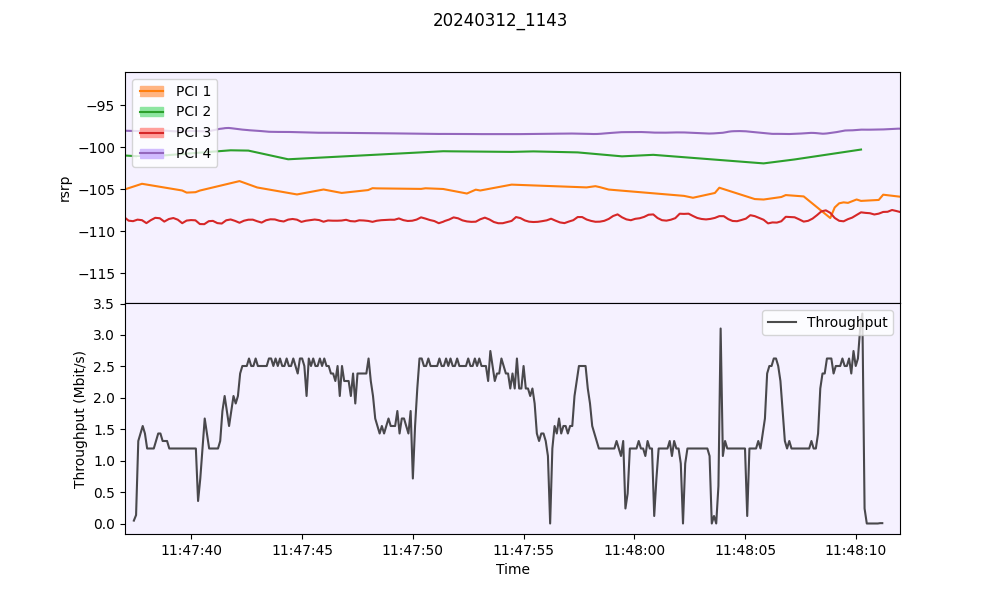
\includegraphics[width=0.75\linewidth]{src//img/4stationary_udp.png}
    \caption{Stationary UDP Capture}
    \label{fig:4udp}
\end{figure}
\begin{figure}
    \centering
    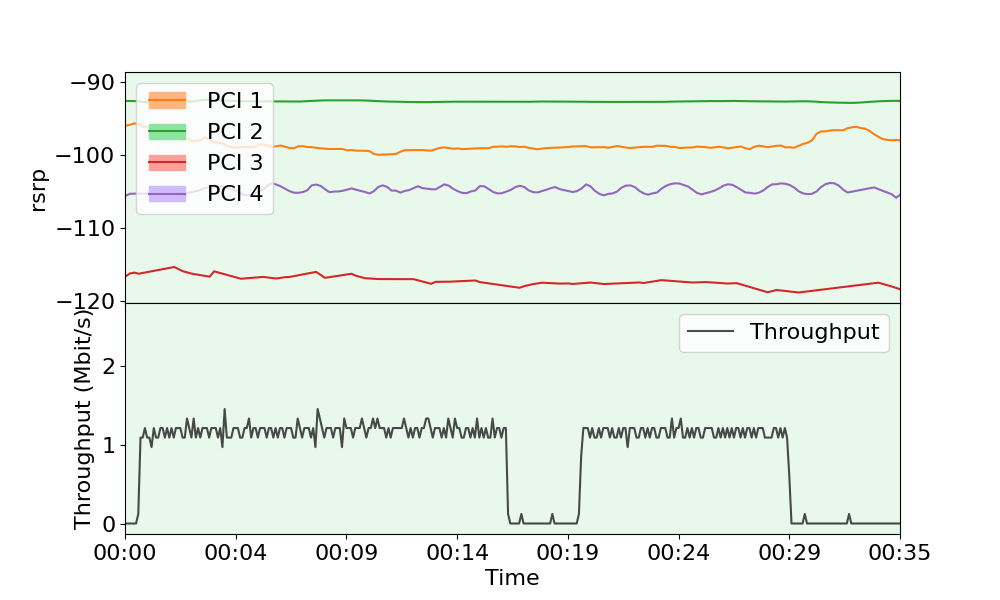
\includegraphics[width=0.75\linewidth]{src//img/4stationary_tcp.png}
    \caption{Stationary TCP Capture}
    \label{fig:4tcp}
\end{figure}

\subsubsection{Immediate Discussion}
Determining the best protocol to use for testing the network proves difficult. UDP provides a better understanding of the maximum throughput the connection can allow. However, due to its ubiquity, TCP better emulates how regular communication is affected by network performance.
Due to the network's inherent instability, TCP becomes unviable when testing our network. As packet loss impacts TCP's communication ability, large outages appear during our throughput measurements. This would limit our understanding of the effect of HO on throughput. Furthermore, we wish to test the network's maximum capacity, so UDP provides a more granular view.

We, therefore, use UDP in our following experiments.

\subsection{Increasing cell density}

\subsubsection{Objective}
The previous mobility tests were run with only two eNBs enabled. This does not fully represent planned indoor deployments; many will use higher cell density. This experiment focuses on the network's performance with more active cells. We can hypothesise that the handover rate will be much higher with increasing cell density (more eNBs enabled).

\subsubsection{Approach}
We reenact the walking mobility test from Experiment \ref{sec:exp:real:mobile} over multiple captures. In this experiment, we enable all four eNBs. To generate a more natural data sample. we move around the lab without a specific path to emulate wandering around.

Considering our conclusion from the previous experiment, we enable UDP throughput capture.
\subsubsection{Results}
The experiment's results are shown in Figures \ref{fig:real:4enb:walk:sup1} and \ref{fig:real:4enb:walk:sup2}. Here, we observed a set of figures without the expected clear throughput drop during a handover event; instead, the throughput was not steady enough to draw such conclusions.

Many handovers occur during each experiment, between 2 and 3 handovers per minute. Furthermore, we see the appearance of ping-pong handovers occurring in Figures \ref{fig:real:4enb:walk:1} and \ref{fig:real:4enb:walk:2}. In Figure \ref{fig:real:4enb:walk:1}, the handover at 00:31 lasts 40ms, and the handover at 02:40 lasts 153ms. In Figure \ref{fig:real:4enb:walk:2} the handover at 00:57 lasts 57ms.

To better understand the figures, we calculate Pearson's Correlation Coefficient between the RSRP of the connected cell and the throughput. We additionally calculate the mean throughput by eNB. These are presented in Table \ref{tab:exp:4enb}.

\begin{figure}
    \centering
    \caption{Moving Capture of Throughput (1)}
    \label{fig:real:4enb:walk:sup1}
    \begin{subfigure}{\linewidth}
        \centering
        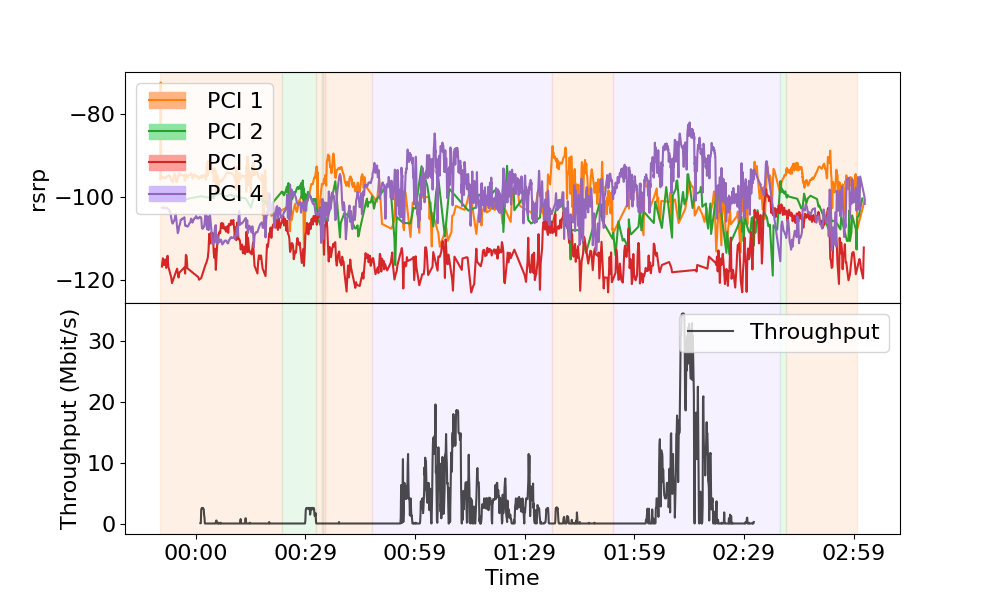
\includegraphics[width=0.9\linewidth]{src/img/4NEW1.png}
        \caption{Capture 1}
        \label{fig:real:4enb:walk:1}
    \end{subfigure}
    \begin{subfigure}{\linewidth}
        \centering
        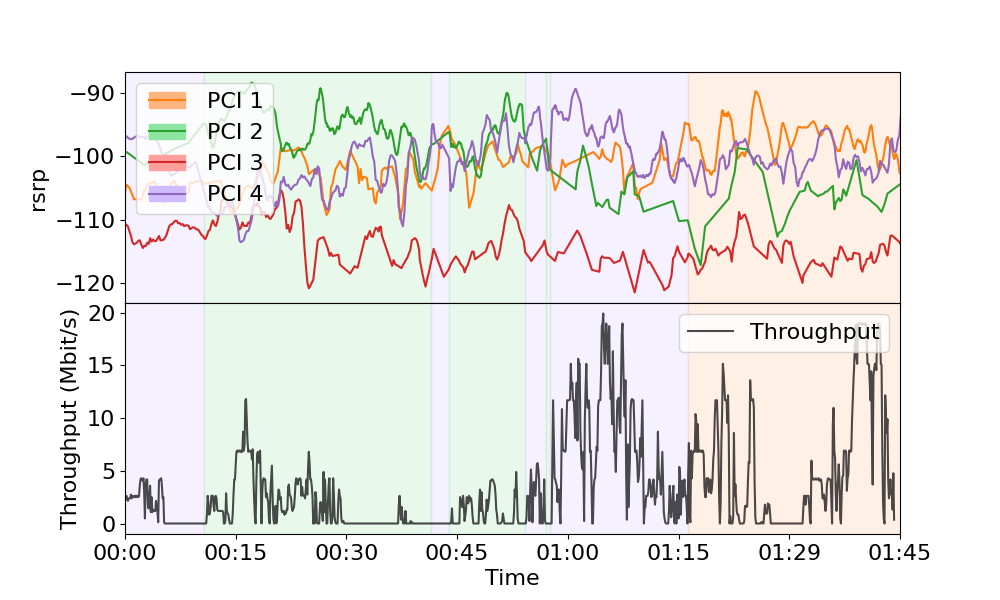
\includegraphics[width=0.9\linewidth]{src/img/3NEW2.png}
        \caption{Capture 2}
        \label{fig:real:4enb:walk:2}
    \end{subfigure}
\end{figure}

\begin{figure}
    \centering
    \caption{Moving Capture of Throughput (2)}
    \label{fig:real:4enb:walk:sup2}
    \begin{subfigure}{\linewidth}
        \centering
        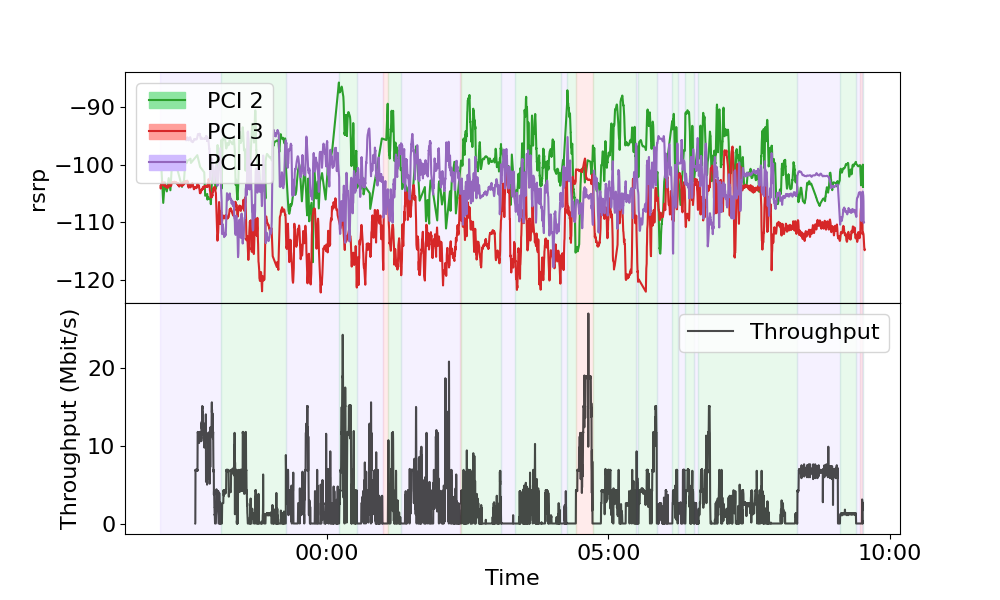
\includegraphics[width=0.9\linewidth]{src/img/3NEW3.png}
        \caption{Capture 3}
        \label{fig:real:4enb:walk:3}
    \end{subfigure}
    \begin{subfigure}{\linewidth}
        \centering
        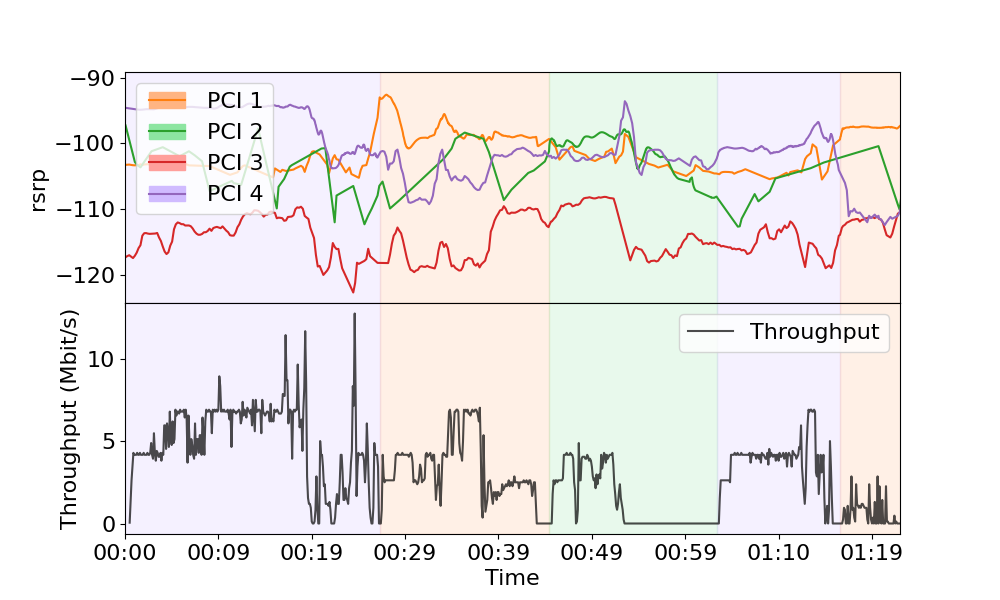
\includegraphics[width=0.9\linewidth]{src/img/3New4.png}
        \caption{Capture 4}
        \label{fig:real:4enb:walk:4}
    \end{subfigure}

\end{figure}

\begin{table}[h]
\caption{Correlations and Throughputs of Experiment}
\label{tab:exp:4enb}
\centering
\begin{tabular}{@{}l|l|llll@{}}
\toprule
&Pearson's&\multicolumn{4}{c}{Mean Throughput (Mbits/s) } \\
         & Correlation & PCI 1 & PCI 2 & PCI 3 & PCI 4 \\ \midrule
Figure \ref{fig:real:4enb:walk:1} & 0.55                  & 0.12            & 0.50             & 0.00             & 4.56            \\
Figure \ref{fig:real:4enb:walk:2} & 0.13                 & 6.05            & 1.73            & 0.00              & 4.08            \\
Figure \ref{fig:real:4enb:walk:3} & 0.04                 & 0.00             & 2.47            & 9.21            & 3.52            \\
Figure \ref{fig:real:4enb:walk:4} & 0.50                  & 2.74            & 1.60             & 0.00              & 4.34            \\ \bottomrule
\end{tabular}
\end{table}

\subsubsection{Immediate Discussion}
In all four captures, we see a high rate of handover even when the signal quality has not significantly fallen. This observation is primarily due to the increased density of eNBs with similar signal strengths. Two of the captures have ping-pong handovers, where a handover occurs within a few seconds of the initial handover.

The throughput instability makes analysis very difficult. This is seen in Table \ref{tab:exp:4enb}, where there is a great disparity between the throughputs of the different eNBs. While there is a moderate correlation between the signal strength (RSRP) and the throughput in two of the experiments (0.55 and 0.50), the other two experiments do not present this relationship (0.13 and 0.04).



% ===========================End Varying Cell Density================================ %

\subsection{Hysteresis Impact}
\subsubsection{Objective}
During the previous experiments, we saw a very high rate of handovers, even when throughput was not improved. We turn to our tuneable parameters of handover: TTT and hysteresis. Considering our results from Experiment \ref{sec:exp:custom}, we can hypothesise that Hysteresis will most impact our ping-pong and handover rate.

\subsubsection{Approach}
To determine the effect of hysteresis on handover, we run a series of experiments adjusting the hysteresis value. We can set up the experiment with 4 eNBs enabled and the UE stationary, positioned so that the RSRP values of the eNBs are similar, where the chance of a ping-pong handover is high. We run the experiment with hysteresis values of 0, 3dBm, 6dBm and 9dBm.

\subsubsection{Results}
The experiment results are plotted in Figure \ref{fig:methods:hysteresis}. We see the rate of handover decrease for each increase in the threshold. We see a rate of 1.73 handovers/min for a 0dBm margin, 0.68 handovers/min for a 3dBm margin,  0.21 handovers/min for a 6dBm margin and 0.12 handovers/min for a 9dBm margin.

\begin{figure}[p]
    \centering
    \caption{Hysteresis values effects on HO rate}
    \label{fig:methods:hysteresis}
    \begin{subfigure}{\linewidth}
        \centering
        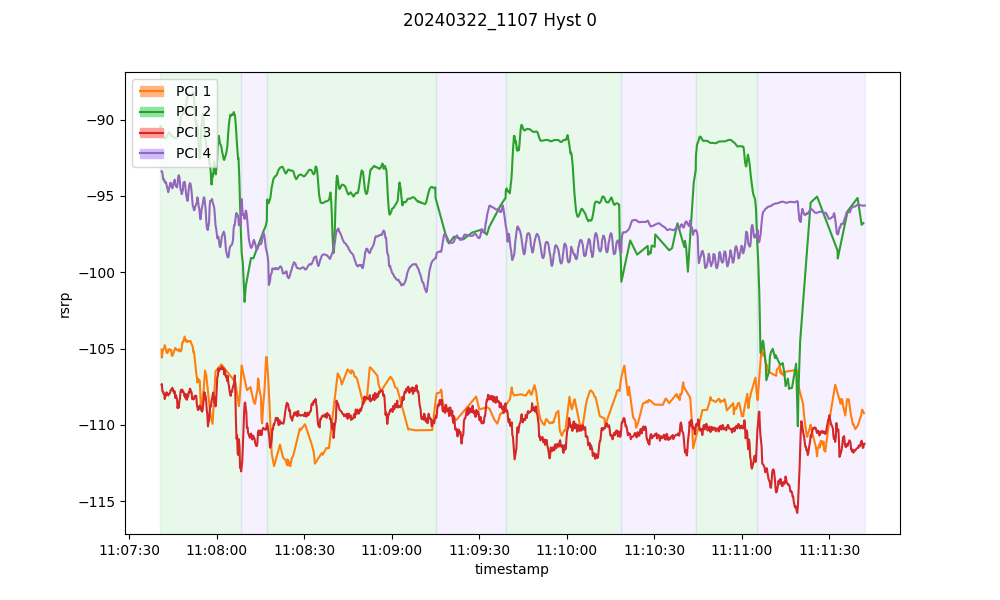
\includegraphics[width=0.55\linewidth]{src//img/5hyst0.png}
        \caption{Hysteresis Threshold: 0dBm}
        \label{fig:methods:hyst0}
    \end{subfigure}
    
    \begin{subfigure}{.9\linewidth}
        \centering
        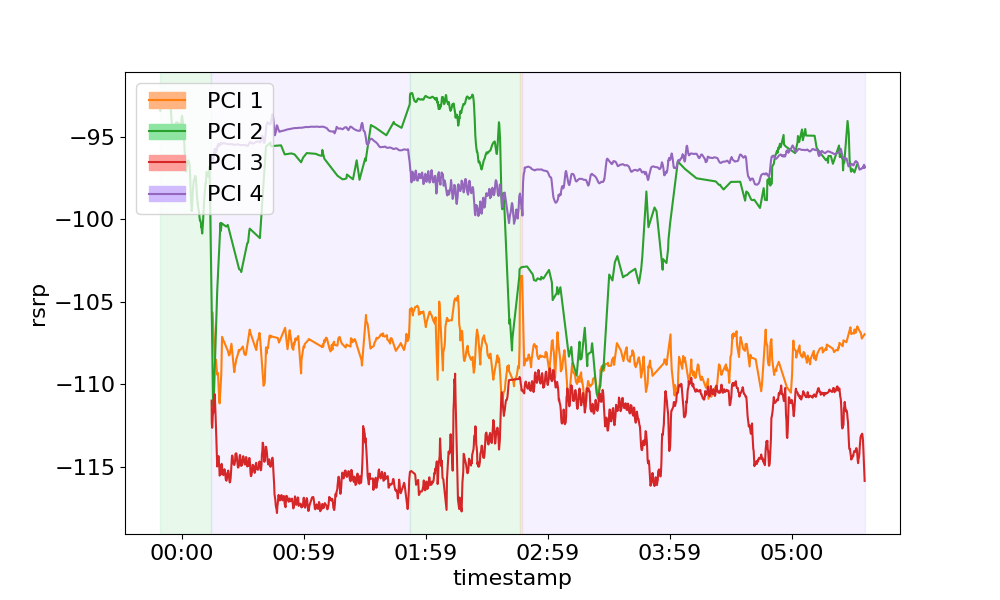
\includegraphics[width=0.6\linewidth]{src//img/5hyst3.png}
        \caption{Hysteresis Threshold: +3dBm}
        \label{fig:methods:hyst3}
    \end{subfigure}
    
    \begin{subfigure}{\linewidth}
        \centering
        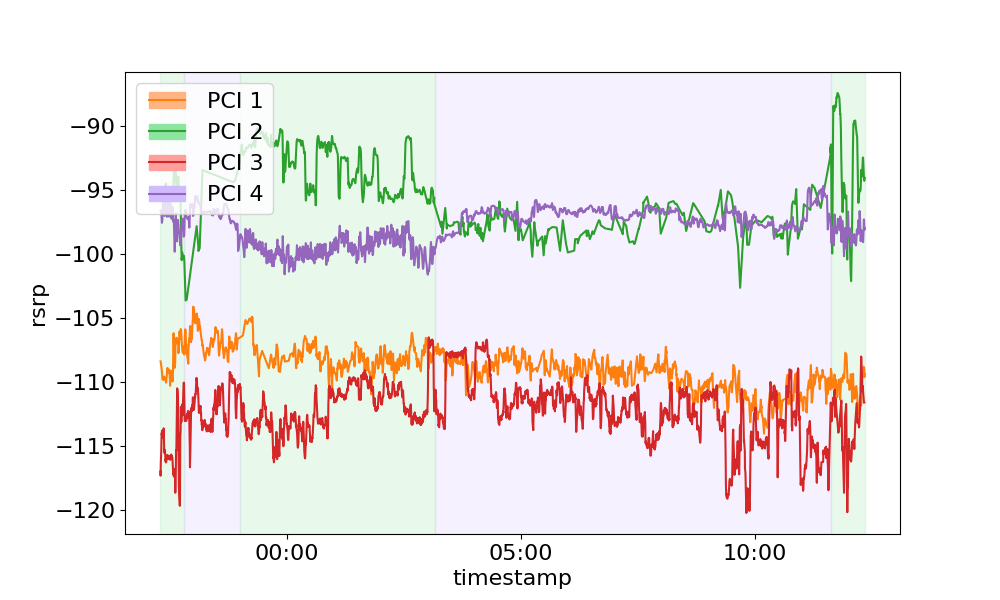
\includegraphics[width=0.55\linewidth]{src//img/5hyst6.png}
        \caption{Hysteresis Threshold: +6dBm}
        \label{fig:methods:hyst6}
    \end{subfigure}
    
    \begin{subfigure}{\linewidth}
        \centering
        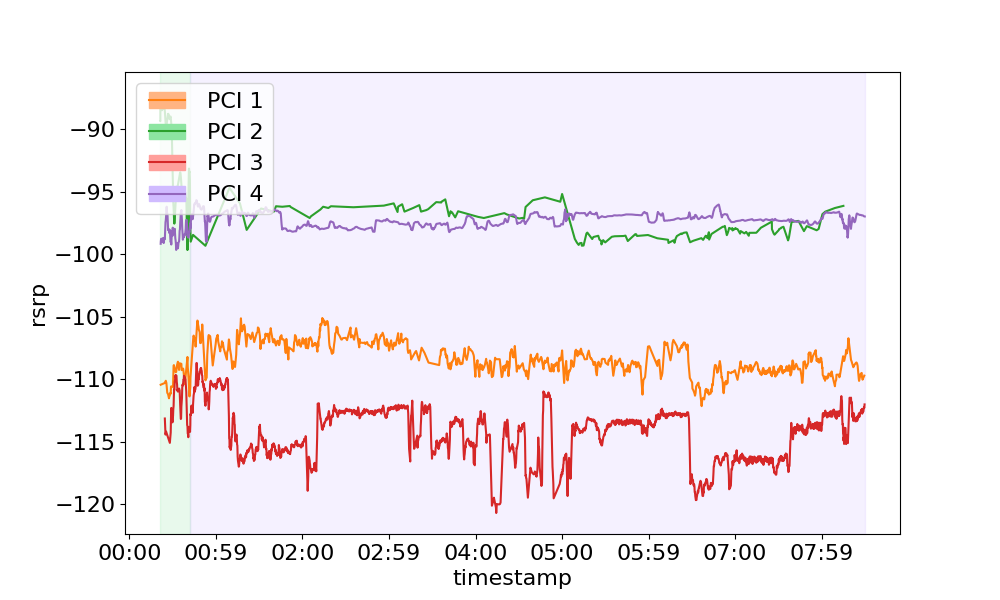
\includegraphics[width=0.55\linewidth]{src//img/5hyst9.png}
        \caption{Hysteresis Threshold: +9dBm}
        \label{fig:methods:hyst9}
    \end{subfigure}
\end{figure}

\subsubsection{Immediate Discussion}
These results are in line with what we have expected. The hysteresis parameter is introduced in network systems to avoid ping-pong handovers specifically. We know from Equation \ref{eq:hysteresis} (simplified) that handover occurs when:
\begin{equation*}
     \text{RSRP}_\text{Target} - \text{RSRP}_\text{Source} > \text{Hysteresis}
 \end{equation*}
 This equates to the two RSRP values being more distinct before the handover is triggered, leading to fewer cases where handover is triggered. Our experimental data supports this; we have a clear relationship between the rate of handover and the hysteresis value.

 While a higher hysteresis value is desirable in this setting to reduce the number of handovers, it negatively impacts other mobility settings, as a higher margin means that handovers will be triggered later and may suffer a throughput penalty before connecting to an eNB with a stronger connection.